% Imporditud: tools/import_eksperimendid.py
% Allikas: Eesti füüsikaolümpiaadi eksperimendi ülesannete
%   kogu (Rael Kalda, 2023), ülesanne Ü159, lahendus L159.
\setAuthor{Eero Uustalu}
\setRound{lõppvoor}
\setYear{2022}
\setNumber{G E1}
\setDifficulty{4}
\setTopic{elektriahelad}
\setVahendid{must kast, millest on välja toodud sinine ja kollane juhe ning mille sees on kaks dioodi ja takistit ühendatud nii, nagu on näidatud juuresoleval skeemil; patarei; multimeeter; samasugune diood nagu mustas kastis, mis on kokku ühendatud takistiga takistusega ligikaudu $R = \SI{2,43}{k\ohm}$. Takisti ja dioodi vabade otste külge on ühendamise hõlbustamiseks külge joodetud juhtmejupid ning takisti ja dioodi ühenduskoha külge on võimalik kinnitada juhe või krokodill}
\setPunktid{12}
\setAllikas{Eksperimendi kogu Ü159, lahendus lk 119}
\setLahendusseis{toores}

\prob{Must kast}
Leida võimalikult täpselt mustas kastis olevate takistite $R_1$ ja $R_2$
väärtused!

\begin{center}
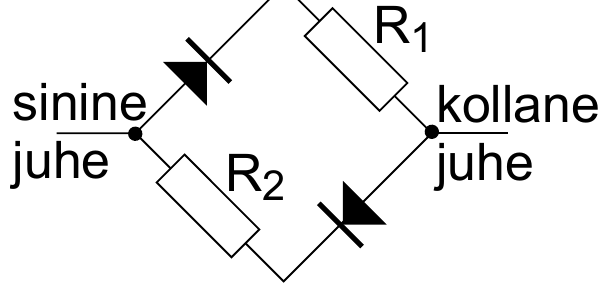
\includegraphics[width=0.45\linewidth]{2022-v3g-ge1-yl.png}
\end{center}

\textit{Vihje:} dioodi läbiv vool sõltub rakendatud pingest mittelineaarselt,
kusjuures vastupinge rakendamisel (st siis, kui vool peaks liikuma noolele
vastassuunas) on voolutugevus tühiselt väike.

\textbf{NB!} Mitte ühendada dioodi otse patarei klemmidele, selle tulemusel
hävineb diood või põleb sisse patareipesa.

\hint

\solu
Ühendame dioodi ja tuntud takisti järjestikku musta kastiga nii, et pluss-klemm on sinise juhtme küljes. Mõõdame pinge dioodil Ud, pinge takistil Ut ning pinge mustal kastil Um. Voolutugevus ahelas $I_1$ = Ut/R läheb läbi takisti $R_1$ ning pinge selle takistil leiame kui musta kasti pinge ning dioodi pinge vahe ($R_1$ juures olev diood ning eraldiolev diood ja neid läbivad voolud on ühesugused, seega on ühesugused ka nende pinged): UR1 = Um $-$ Ud, millest $R_1$ = (Um $-$ Ud)/$I_1$ = (Um $-$ Ud)R/Ut. Analoogselt leiame takisti $R_2$ väärtuse pöörates patarei vastupidi: $R_2$ = (Vm $-$ Vd)/$I_2$ = (Vm $-$ Vd)R/Vt, kus Vm, Vd ja Vt tähistavad vastavaid pingeid uues olukorras.
\probend
